\EnglishSourceFrame{GELFAND-P001475}{70}
The Hessian is a quadratic form on the space (13), invariantly
defined at a critical point.
\begin{equation*}
H(\varphi)=\int_M\operatorname{Tr}(\nabla_{ad}\varphi\cdot\varphi),
\qquad \varphi\in T_{X,\nabla}, \tag{14}
\end{equation*}
\begin{equation*}
\Omega^1(M)\otimes\mathrm{su}_2
\overset{\nabla_{ad}}{\longrightarrow}
\Omega^2(M)\otimes\mathrm{su}_2. \tag{15}
\end{equation*}
If the connection was integrable, then $\nabla_{ad}$ is a complex
([a sign is crossed out:
\EnglishUnclear{GELFAND-P001475}{complex-cancel}{$\varphi$ / $\Phi$ / illegible}]
$\nabla_{ad}^{2}=0$)
and $\nabla_{ad}\varphi$ is well defined (independent of the representative
in the quotient (13)).

\underline{The function} [inserted above the line:
\EnglishUnclear{GELFAND-P001475}{morse-function-insert}{$\int\nu$ / $\int v$}]
\underline{is Morse} $\Longleftrightarrow$ $\nabla_{ad}$ has no
cohomology in degree 1, i.e.
\begin{equation*}
H^1(M,\text{any representation of }\pi_1)=0 \tag{16}
\end{equation*}
[Below “any representation of $\pi_1$” is added: “or $\forall$ local syst. [source abbreviation]”]

This is equivalent to
\begin{equation*}
M\text{ --- a homology sphere, i.e. }H_1(X,\mathbb Z)=0 \tag{17}
\end{equation*}
\EnglishUnclear{GELFAND-P001475}{homology-equivalence}{[In (17), $X$ is written; the equivalence claim is retained as in the source.]}

Following the standard scheme, one should consider gradient flows.

2 critical points $\longleftrightarrow$ 2 representations of $\pi_1$.

Join them by a trajectory of nonintegrable connections.

Choose a single coordinate system in a neighborhood of the curve
\begin{center}
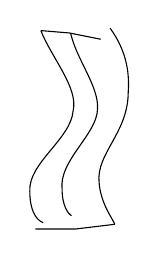
\begin{tikzpicture}[x=1cm,y=1cm]
\draw (0.04,2.50) .. controls (0.18,2.15) and (0.52,1.77) .. (0.45,1.48)
 .. controls (0.42,1.12) and (-0.12,0.82) .. (-0.10,0.46)
 .. controls (-0.10,0.23) and (-0.03,0.10) .. (0.07,0.06);
\draw (0.92,2.53) .. controls (1.11,2.27) and (1.17,2.00) .. (1.15,1.72)
 .. controls (1.15,1.20) and (0.74,0.94) .. (0.78,0.57)
 .. controls (0.80,0.31) and (0.94,0.13) .. (0.98,0.04);
\draw (0.04,2.50) -- (0.40,2.47) -- (0.80,2.39);
\draw (0.42,2.46) .. controls (0.50,2.12) and (0.78,1.79) .. (0.76,1.50)
 .. controls (0.75,1.18) and (0.27,0.85) .. (0.31,0.49)
 .. controls (0.31,0.27) and (0.39,0.17) .. (0.43,0.15);
\draw (-0.03,-0.02) -- (0.48,-0.02) -- (0.98,0.04);
\end{tikzpicture}
\end{center}
and follow the change in the matrix of second derivatives.
\begin{equation*}
\begin{aligned}
\text{Difference [inserted: of indices]}&=
\text{number of points [inserted: along the path] where a zero mode appears}\\
&=\text{spectral asymmetry.}
\end{aligned}\tag{18}
\end{equation*}
This is done with
\EnglishUnclear{GELFAND-P001475}{index-theorem-cancel}{[An illegible crossed-out word]}
the aid of the usual index theorem.
\begin{equation*}
\text{Difference of indices, }\underline{\mathrm{mod}\ 8},\quad
\text{is well defined!!} \tag{19}
\end{equation*}

\EnglishSourceFrame{GELFAND-P001476}{unlabelled}
\underline{The next example.}

Calculating the index from the viewpoint of the finite-dimensional situation.
(Again for a homology sphere.)

\begin{center}
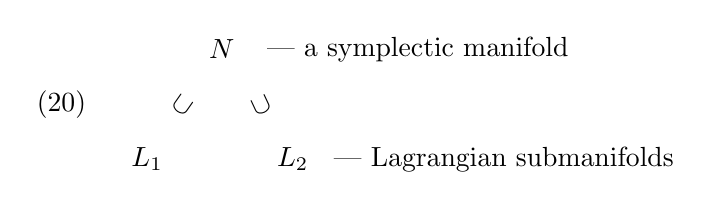
\begin{tikzpicture}[x=1cm,y=1cm]
\node at (0,1.4) {$N$};
\node[anchor=west] at (0.45,1.4) {--- a symplectic manifold};
\node[rotate=-35] at (-0.50,0.68) {$\cup$};
\node[rotate=25] at (0.50,0.68) {$\cup$};
\node at (-0.95,0) {$L_1$};
\node at (0.90,0) {$L_2$};
\node[anchor=west] at (1.30,0) {--- Lagrangian submanifolds};
\node[anchor=east] at (-1.60,0.7) {(20)};
\end{tikzpicture}
\end{center}
Let
\begin{equation*}
L_1\cap L_2\quad\text{is finite.}\tag{21}
\end{equation*}
We want to calculate the weighted number of intersection points.

(22) \underline{Example.} $N=$
\EnglishUnclear{GELFAND-P001476}{cotangent-cancel}{[Crossed out: $\Omega$ / an illegible sign]}
$T^*L$,
\begin{center}
\begin{tikzcd}[column sep=large]
L_1=L \arrow[r,hook,"{\text{zero section}}"] & N &
L=L_2 \arrow[l,hook',"df"]
\end{tikzcd}
\end{center}
[Below $L_1=L$, crossed out:
\EnglishUnclear{GELFAND-P001476}{below-section-cancel}{$H_2$ / $L_2$ / illegible}.]
$f$ is Morse

$L_1\cap L_2$ are the critical points of $f$

the intersection is transverse.

An intersection point is assigned an index
\begin{equation*}
L_1\cap L_2\overset{\mathrm{index}}{\longrightarrow}
\{0,1,\ldots,\dim L\}
\end{equation*}
\begin{equation*}
\chi(N)=\sum_{x\in L_1\cap L_2}(-1)^{\mathrm{index}\,x}\tag{23}
\end{equation*}
\underline{The general situation (20)}: define a relative index!

(24) $X$ is the space of paths joining $L_1$ and $L_2$
\begin{equation*}
\begin{aligned}
[0,1]&\longrightarrow N\\
0&\longrightarrow L_1\\
1&\longrightarrow L_2
\end{aligned}
\end{equation*}
On such an $X$ there is a multivalued Morse function

The critical points are the intersection points of $L_j$

$\varphi\in X$, $\tau$ is a tangent vector at $\varphi$, i.e. a vector field along $\varphi$

[A short line leads down from $\varphi$ to the caption “path”.]

\EnglishSourceFrame{GELFAND-P001477}{71}
Then
\begin{equation*}
\langle \nu,\tau\rangle := \int_0^1 \omega(\dot{\varphi},\tau),
\tag{25}
\end{equation*}
\EnglishUnclear{GELFAND-P001477}{one-form-symbol}{The sign rendered as $\nu$ may be Latin $v$; the same sign stands below before “Morse”.}

where

$\omega$ is the symplectic form.

$\nu$ is Morse if $L_1$ and $L_2$ intersect transversely.

The difference of indices is defined, but there is also an elementary construction

(through the Maslov index)

Consider a manifold $M$, a homology sphere. !

(26) \underline{Theorem}

$M$ can be cut along a Riemann surface $Z$,

(a Heegaard splitting)

$$
W=W_1\cup W_2,\qquad \partial W_i=Z.
$$
\EnglishUnclear{GELFAND-P001477}{decomposition-letter}{The formula has $W$, whereas the preceding text has $M$; their relation is not explained.}

(27)
\begin{center}
\begin{tikzcd}[row sep=small,column sep=large]
& \pi_1(W_1) \arrow[dr] & \\
\pi_1(Z) \arrow[ur] \arrow[dr] & & \pi_1(M) \\
& \pi_1(W_2) \arrow[ur] &
\end{tikzcd}
\end{center}

together determine $\pi_1(M)$

$\pi_1(W_j)$ is a free group on $g$ generators

Representations of $\pi_1(M)$ [crossed out: \EnglishUnclear{GELFAND-P001477}{cancelled-representation-word}{one illegible word}]
--- within it, $\pi_1(W_j)$ are Lagrangian manifolds.

Consider

(28)
\EnglishSourceFigure{GELFAND-P001477}{cylinder-decomposition}{A horizontal drawing: two convex outer parts are joined above and below by nearly straight lines. Arcs, some faint, are visible at the joins. Above the left part is $W_1$, above the right part $W_2$, and below the middle part “cylinder”. Short sloping strokes at the upper joins do not confidently establish whether they are arrows or part of the outline.}

\par\medskip\noindent
\begin{minipage}[c]{0.48\linewidth}\centering
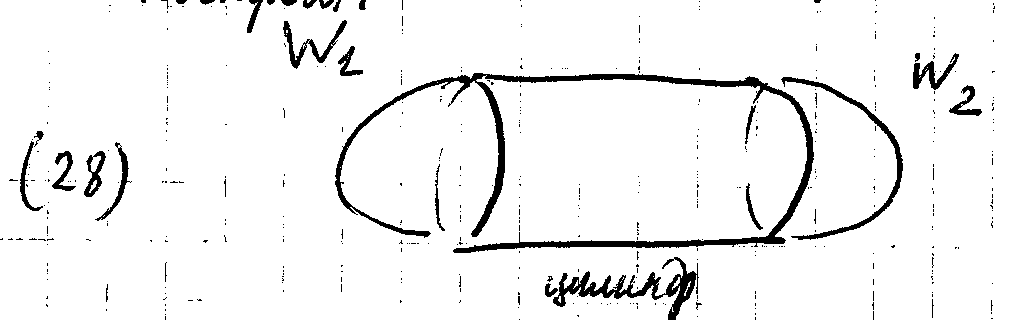
\includegraphics[width=\linewidth]{figures/gelfand-p001477-cylinder-decomposition-original.png}
\par\smallskip{\footnotesize Original manuscript diagram: GELFAND-P001477\par}
\end{minipage}\hfill
\begin{minipage}[c]{0.48\linewidth}\centering
\resizebox{\linewidth}{!}{% Partial visible-stroke recreation; uncertain connectivity remains open.
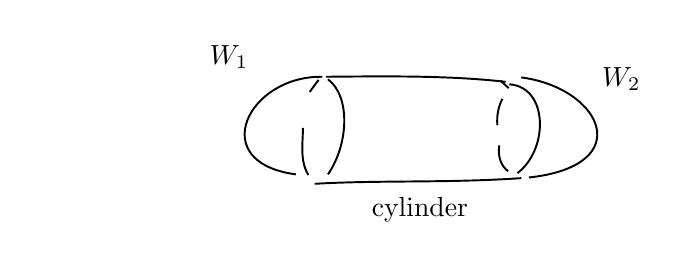
\begin{tikzpicture}[x=0.008cm,y=-0.008cm,line width=0.7pt]
\path[use as bounding box] (0,0) rectangle (1020,320);
\draw (468,78)..controls(350,76)and(282,214)..(426,233);
\draw (477,82)..controls(513,109)and(510,185)..(477,233);
\draw (446,234)..controls(431,211)and(438,178)..(437,159);
\draw (474,78)..controls(574,77)and(671,76)..(759,86);
\draw (456,248)..controls(558,242)and(667,247)..(784,239);
\draw (784,79)..controls(912,96)and(970,219)..(796,238);
\draw (765,90)..controls(827,94)and(828,193)..(778,231);
\draw (754,113)..controls(747,127)and(745,140)..(746,155);
\draw (749,187)..controls(746,208)and(754,221)..(763,228);
\draw (462,83)--(448,102);\draw (751,84)--(764,96);
\node at (320,47) {$W_1$};\node at (943,82) {$W_2$};
\node at (623,289) {cylinder};
\end{tikzpicture}
}
\par\smallskip{\footnotesize Partial recreation; unclear joins, crossings and arrowheads remain unresolved.\par}
\end{minipage}\par\medskip


[Crossed out: \EnglishUnclear{GELFAND-P001477}{cancelled-before-path}{one illegible word before “Path”}]
A path is a family of connections.

The second half of the work:

replacing flat connections by instantons,

passing to $M^4$ and

Donaldson invariants

($M^4$ is cut into 2 three-dimensional ones).
\EnglishUnclear{GELFAND-P001477}{four-dimensional-cut}{The phrase “$M^4$ is cut into 2 three-dimensional ones” is rendered literally; its dimensional meaning is not specified.}

\EnglishSourceFrame{GELFAND-P001478}{unlabelled}
\underline{12.9.88.}\qquad \underline{\underline{Gelfand's seminar.}}

1. “What is the smallest number of dimensions of a space in which two
two-dimensional planes can be skew?”

2. \underline{\underline{What is a determinant?}}

Two first-order equations can be replaced [inserted above the line: by one]
second-order equation. How?

\begin{equation*}
\begin{cases}
\left(\dfrac{d}{dx}+q_{11}\right)\varphi_1+q_{12}\varphi_2=0\\
q_{21}\varphi_1+\left(\dfrac{d}{dx}+q_{22}\right)\varphi_2=0
\end{cases}
\tag{1}
\end{equation*}

a) \underline{First method}: express $\varphi_2$ from the first equation and substitute into the second

\underline{Second method}: express $\varphi_1$ from the second equation and substitute into the first

Different equations result!

but after solving one, one can solve the second.

This is known as the “Backlund transformation”.

One can take a linear combination of $\varphi_1$ and $\varphi_2$, producing a family of equations.

The answers are very beautiful

b) What about three first-order equations?

This is already more complicated and the beauty disappears.

Done by Gelfand and Retakh.

There is work by Sato and Kashiwara on noncommutative determinants.

c) Let $q_{ij}=\mathrm{const}$

[Crossed out on the left: \EnglishUnclear{GELFAND-P001478}{cancelled-margin-label}{an illegible item label with a right parenthesis}]
Then there is a determinant

\begin{equation*}
\begin{vmatrix}
\dfrac{d}{dx}+q_{11}&q_{12}\\
q_{21}&\dfrac{d}{dx}+q_{22}
\end{vmatrix}
=\left(\frac{d}{dx}\right)^2+(q_{11}+q_{22})\frac{d}{dx}
+(q_{11}q_{22}-q_{12}q_{21})
\tag{2}
\end{equation*}

$$
\frac{d}{dx}\longleftrightarrow\lambda
\qquad\Longrightarrow\qquad\text{gives the characteristic determinant of the matrix}
$$

In the general case one obtains [inserted above the line: (a noncommutative analogue)]
of the characteristic determinant.

$$
\begin{vmatrix}
a_{11}&a_{12}\\
a_{21}&a_{22}
\end{vmatrix}
\quad\text{--- ?}
$$

$a_{ij}$ is a map $E_j\to E_i$,

so $a_{11}a_{22}-a_{12}a_{21}$ has no meaning.

There are four determinants in all:

\begin{equation*}
a_{11}-a_{12}a_{22}^{-1}a_{21}
\tag{3}
\end{equation*}

[Crossed out: \EnglishUnclear{GELFAND-P001478}{cancelled-final-symbol}{one sign resembling $a$ or Cyrillic i}]
and so on.

\EnglishSourceFrame{GELFAND-P001479}{84}
Third order: 36 ways of writing it.

Noncommutative $K$-theory and noncommutative homology arise.

\EnglishUnclear{GELFAND-P001479}{overwritten-section-label}{c) / d)}
Eight letters are arranged in a $2\times2\times2$ cube

What is the determinant?

This was done by Cayley.

It was thought that after Hilbert, the results of Gordan, Cayley, Clebsch and others
had lost their interest. They were declared old-fashioned nonsense. But this
is wrong.

\underline{\underline{Moore.}}\quad (\underline{GREGORY MOORE})\quad (\underline{I,AS. Princeton})

\underline{Conformal} \underline{field} \underline{theory.}\quad (CFT)

The Ising model

\begin{center}
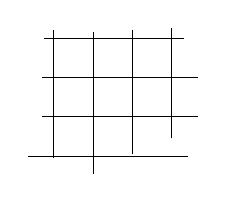
\begin{tikzpicture}[scale=0.5]
\draw (0,-0.05)--(0,3.2);
\draw (1,-0.45)--(1,3.15);
\draw (2,0.05)--(2,3.2);
\draw (3,0.45)--(3,3.25);
\draw (-0.25,3)--(3.3,3);
\draw (-0.3,2)--(3.65,2);
\draw (-0.3,1)--(3.65,1);
\draw (-0.65,0)--(3.4,0);
\end{tikzpicture}
\end{center}

A 2-dimensional lattice, at $\forall$ point a variable $\sigma :=$
[crossed out: \EnglishUnclear{GELFAND-P001479}{cancelled-spin-value}{a short entry covered by dense sloping strokes}] $\pm1$

[Below “lattice”: (square)]

\begin{equation*}
\text{Energy}\quad E=\sum_{\langle ij\rangle}\sigma_i\sigma_j
\tag{1}
\end{equation*}

$\langle ij\rangle$ are neighboring points

Partition function

\begin{equation*}
Z=\sum e^{-\beta E}
\tag{2}
\end{equation*}

\EnglishSourceFigure{GELFAND-P001479}{ising-cylinder}{A vertical cylinder: a closed upper oval, two side lines and a lower arc. Several nearly vertical lines run inside; at the bottom are a short sloping stroke on the left and a transverse stroke farther right. The exact joining of the internal lines and the meaning of the short strokes are unclear; the drawing has no labels.}

\par\medskip\noindent
\begin{minipage}[c]{0.48\linewidth}\centering
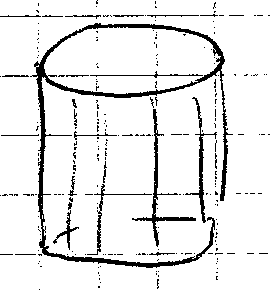
\includegraphics[width=\linewidth]{figures/gelfand-p001479-ising-cylinder-original.png}
\par\smallskip{\footnotesize Original manuscript diagram: GELFAND-P001479\par}
\end{minipage}\hfill
\begin{minipage}[c]{0.48\linewidth}\centering
\resizebox{\linewidth}{!}{% Partial visible-stroke recreation; uncertain connectivity remains open.
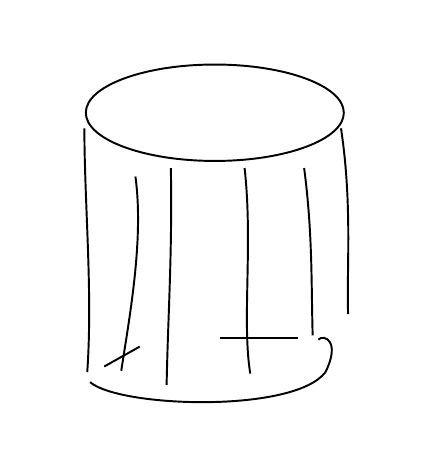
\begin{tikzpicture}[x=0.018cm,y=-0.018cm,line width=0.7pt]
\path[use as bounding box] (0,0) rectangle (270,290);
\draw (132,60) ellipse[x radius=91,y radius=34];
\draw (40,71)..controls(40,124)and(46,187)..(42,243);
\draw (221,71)..controls(229,124)and(225,168)..(226,202);
\draw (44,250)..controls(65,268)and(188,272)..(210,243);
\draw (210,243)..controls(221,221)and(209,216)..(205,220);
\draw (76,105)..controls(82,149)and(72,203)..(66,242);
\draw (101,99)..controls(102,162)and(99,201)..(98,252);
\draw (153,99)..controls(159,153)and(151,207)..(157,244);
\draw (195,99)..controls(201,145)and(200,180)..(201,217);
\draw (54,239)--(79,225);\draw (136,219)--(191,219);
\end{tikzpicture}
}
\par\smallskip{\footnotesize Partial recreation; unclear joins, crossings and arrowheads remain unresolved.\par}
\end{minipage}\par\medskip


Consider it on a cylinder and refine the lattice

The asymptotics are expressed through the functions

[Crossed out on the left: \EnglishUnclear{GELFAND-P001479}{cancelled-before-eta}{a sign resembling $Z$, followed by illegible strokes}]

$$
\eta(\tau)=q^{1/24}\prod(1-q^n),\qquad q=e^{i\pi\tau}
$$
\EnglishUnclear{GELFAND-P001479}{eta-q-normalization}{The source has $q=e^{i\pi\tau}$ together with $q^{1/24}\prod(1-q^n)$; compatibility of the normalizations is not specified.}

$$
\theta_3(\tau)=\sum e^{i\pi\tau n^2}
$$

and similarly $\theta_2,\theta_4$

[Above the line: $\tau=i\beta$]

Invariant under the substitution

$$
\tau\longrightarrow-1/\tau
$$

$$
Z\longrightarrow
\left|\frac{\theta_2}{\eta}\right|
+\left|\frac{\theta_3}{\eta}\right|
+\left|\frac{\theta_1}{\eta}\right|
\qquad\text{(up to a factor)}
$$
\EnglishUnclear{GELFAND-P001479}{last-theta-index}{The last index most closely resembles $1$; possibly $4$. Above, $\theta_2,\theta_4$ are written separately.}

$$
Z(\beta)=Z\left(\frac{1}{\beta}\right)
$$

\EnglishSourceFrame{GELFAND-P001480}{unlabelled}
In CFT we associate real analytic functions
to surfaces

\EnglishSourceFigure{GELFAND-P001480}{top-torus-cycles}{A torus with a hole; below is an arc labeled $\alpha$, and on the right a transverse arc labeled $\beta$. A leftward head is visible on the lower arc and a downward-right head by the outer outline. Strokes near the upper edge of the hole and gaps in the transverse arc require comparison with the original.}

\par\medskip\noindent
\begin{minipage}[c]{0.48\linewidth}\centering
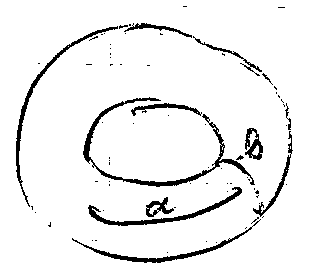
\includegraphics[width=\linewidth]{figures/gelfand-p001480-top-torus-cycles-original.png}
\par\smallskip{\footnotesize Original manuscript diagram: GELFAND-P001480\par}
\end{minipage}\hfill
\begin{minipage}[c]{0.48\linewidth}\centering
\resizebox{\linewidth}{!}{% Partial visible-stroke recreation; uncertain connectivity remains open.
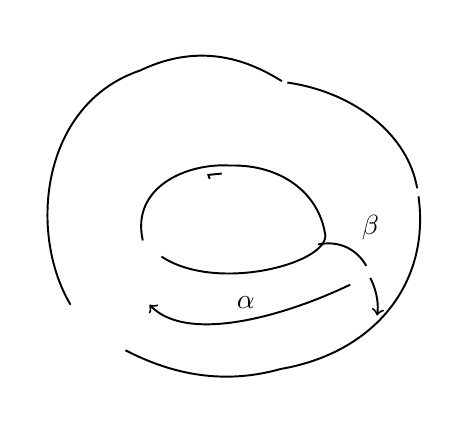
\begin{tikzpicture}[x=0.017cm,y=-0.017cm,line width=0.7pt]
\path[use as bounding box] (0,0) rectangle (310,275);
\draw (32,207)..controls(0,153)and(10,57)..(84,32)
 ..controls(130,10)and(166,25)..(190,40);
\draw (194,41)..controls(243,48)and(284,79)..(291,120);
\draw (292,126)..controls(301,191)and(259,243)..(189,255)
 ..controls(143,268)and(104,257)..(73,241);
\draw (86,159)..controls(77,119)and(119,101)..(151,103)
 ..controls(190,102)and(217,124)..(222,153)
 ..controls(229,175)and(142,199)..(100,171);
\draw (136,113)--(135,110)--(145,109);
\draw[->] (241,192)..controls(191,216)and(119,236)..(91,207);
\draw (217,162)..controls(231,159)and(245,164)..(253,178);
\draw[->] (256,187)..controls(262,199)and(262,209)..(261,215);
\node at (163,205) {$\alpha$};\node at (256,149) {$\beta$};
\end{tikzpicture}
}
\par\smallskip{\footnotesize Partial recreation; unclear joins, crossings and arrowheads remain unresolved.\par}
\end{minipage}\par\medskip

$$
=\sum_{i=1}^{N} f_i(\tau)\bar g_i(\tau),\qquad
f_i:=\left\{\sqrt{\frac{\theta_2}{\eta}},
\sqrt{\frac{\theta_3}{\eta}},
\sqrt{\frac{\theta_4}{\eta}}\right\}
$$
$$
\tau\to-\frac{1}{\tau},\qquad
\begin{pmatrix}f_1\\f_2\\f_3\end{pmatrix}
\to
\begin{pmatrix}0&0&1\\0&1&0\\1&0&0\end{pmatrix}
\begin{pmatrix}f_1\\f_2\\f_3\end{pmatrix}
$$

\underline{Other variants:}

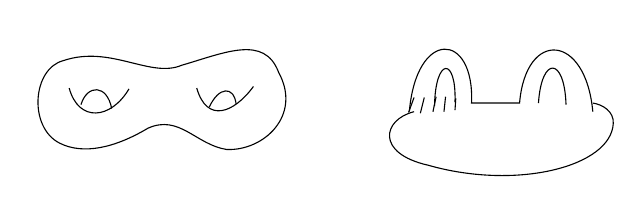
\begin{tikzpicture}[x=1cm,y=1cm]
\draw (0,0) .. controls (-.4,.2) and (-.35,.95) .. (.05,1.05)
.. controls (.65,1.25) and (1.15,.82) .. (1.55,.99)
.. controls (2.1,1.15) and (2.6,1.38) .. (2.78,.9)
.. controls (3.08,.35) and (2.59,-.1) .. (2.12,-.08)
.. controls (1.73,-.02) and (1.52,.37) .. (1.12,.19)
.. controls (.7,-.06) and (.3,-.15) .. (0,0);
\draw (.12,.7) .. controls (.24,.26) and (.65,.3) .. (.88,.69);
\draw (.27,.49) .. controls (.35,.75) and (.6,.75) .. (.66,.44);
\draw (1.74,.7) .. controls (1.87,.25) and (2.21,.38) .. (2.46,.72);
\draw (1.9,.46) .. controls (2.02,.72) and (2.21,.73) .. (2.24,.5);
\draw (4.5,.4) .. controls (4.1,.3) and (4.01,-.13) .. (4.68,-.28)
.. controls (5.8,-.6) and (7,-.3) .. (7.03,.25)
.. controls (7.04,.4) and (6.9,.49) .. (6.77,.51);
\draw (4.44,.4) .. controls (4.53,1.46) and (5.27,1.42) .. (5.23,.51)
-- (5.84,.51) .. controls (5.92,1.45) and (6.68,1.4) .. (6.77,.4);
\draw (4.76,.47) .. controls (4.77,1.1) and (5.04,1.1) .. (5.02,.52);
\draw (6.08,.51) .. controls (6.12,1.11) and (6.41,1.1) .. (6.43,.49);
\draw (4.43,.39)--(4.5,.58);
\draw (4.58,.38)--(4.63,.58);
\draw (4.74,.4)--(4.78,.59);
\draw (4.88,.4)--(4.9,.59);
\draw (5.02,.42)--(5.03,.57);
\end{tikzpicture}

On $\forall$ surface there is a corresponding CFT model!!

\EnglishSourceFigure{GELFAND-P001480}{middle-cut-torus}{A cut torus: two close oval ends at the bottom, $\theta$ below the cut and $\beta$ above. Inside is a curved line and a dense stroke by the left inner edge; whether this is an arrow or a surface line is uncertain.}

\par\medskip\noindent
\begin{minipage}[c]{0.48\linewidth}\centering
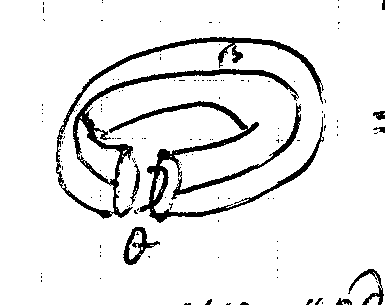
\includegraphics[width=\linewidth]{figures/gelfand-p001480-middle-cut-torus-original.png}
\par\smallskip{\footnotesize Original manuscript diagram: GELFAND-P001480\par}
\end{minipage}\hfill
\begin{minipage}[c]{0.48\linewidth}\centering
\resizebox{\linewidth}{!}{% Partial visible-stroke recreation; uncertain connectivity remains open.
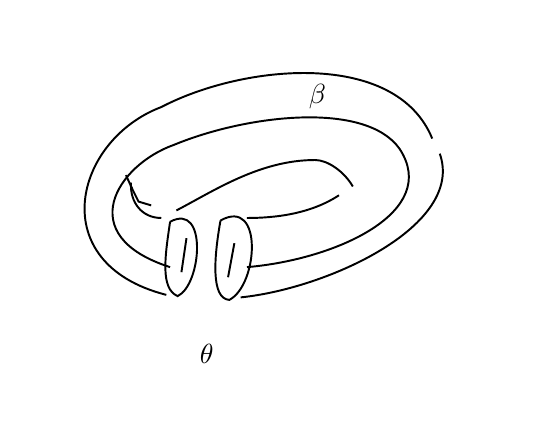
\begin{tikzpicture}[x=0.016cm,y=-0.016cm,line width=0.7pt]
\path[use as bounding box] (0,0) rectangle (385,305);
\draw (110,212)..controls(12,187)and(37,89)..(106,63)
 ..controls(171,29)and(292,17)..(321,88);
\draw (327,100)..controls(347,157)and(238,207)..(169,214);
\draw (113,190)..controls(35,165)and(71,109)..(116,93)
 ..controls(174,69)and(268,58)..(295,96)
 ..controls(328,146)and(245,184)..(174,190);
\draw (118,145)..controls(147,130)and(184,105)..(228,105)
 ..controls(238,105)and(251,114)..(258,126);
\draw (247,133)..controls(224,148)and(196,151)..(174,151);
\draw (106,151)..controls(91,151)and(81,139)..(82,123);
\draw (82,126)--(88,138)--(98,141);\draw (83,128)--(78,117);
\draw (113,154)..controls(143,138)and(138,204)..(119,213)
 ..controls(105,207)and(109,181)..(113,154);
\draw (153,153)..controls(187,134)and(183,204)..(160,216)
 ..controls(145,215)and(148,181)..(153,153);
\draw (126,167)--(122,194);\draw (164,171)--(159,198);
\node at (230,55) {$\beta$};\node at (142,259) {$\theta$};
\end{tikzpicture}
}
\par\smallskip{\footnotesize Partial recreation; unclear joins, crossings and arrowheads remain unresolved.\par}
\end{minipage}\par\medskip

$$
=f(\beta+i\theta,\beta-i\theta)\qquad
\text{(real analytic functions)}
$$
one can twist by $\theta$

The torus parameters are two real numbers
$$\tau=L+i\theta$$

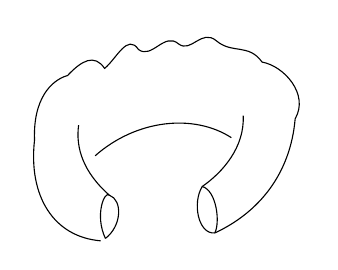
\begin{tikzpicture}[x=1cm,y=1cm]
\draw (.7,0) .. controls (.1,.05) and (-.22,.57) .. (-.14,1.28)
.. controls (-.16,1.8) and (.07,2.04) .. (.28,2.1)
.. controls (.46,2.29) and (.62,2.38) .. (.75,2.19)
.. controls (.9,2.31) and (1.04,2.64) .. (1.18,2.43)
.. controls (1.35,2.3) and (1.51,2.66) .. (1.69,2.5)
.. controls (1.85,2.38) and (1.98,2.7) .. (2.17,2.54)
.. controls (2.37,2.37) and (2.58,2.51) .. (2.75,2.27)
.. controls (3.03,2.22) and (3.35,1.86) .. (3.17,1.55)
.. controls (3.11,.85) and (2.71,.36) .. (2.15,.1);
\draw (.76,.03) .. controls (.97,.19) and (.98,.52) .. (.81,.58)
.. controls (.75,.64) and (.62,.33) .. (.76,.03);
\draw (2.15,.1) .. controls (1.94,.08) and (1.86,.48) .. (1.99,.69)
.. controls (2.17,.64) and (2.22,.24) .. (2.15,.1);
\draw (.81,.58) .. controls (.48,.87) and (.38,1.18) .. (.42,1.47);
\draw (.63,1.08) .. controls (1.15,1.54) and (1.88,1.62) .. (2.36,1.31);
\draw (1.99,.69) .. controls (2.25,.87) and (2.53,1.19) .. (2.51,1.59);
\end{tikzpicture}

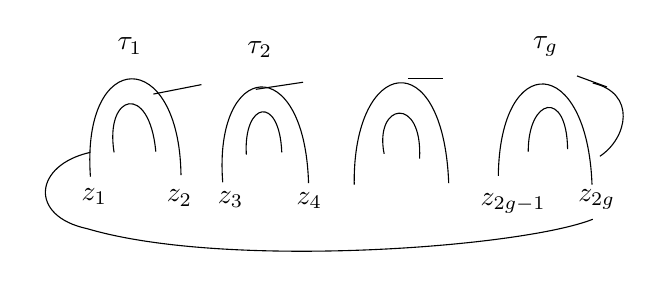
\begin{tikzpicture}[x=1cm,y=1cm]
\draw (0,.45) .. controls (-.72,.29) and (-.79,-.36) .. (-.04,-.52)
.. controls (1.72,-1.04) and (5.47,-.76) .. (6.38,-.4);
\draw (6.47,.4) .. controls (6.82,.63) and (6.94,1.2) .. (6.38,1.33);
\draw (.8,1.19)--(1.41,1.31);
\draw (2.1,1.25)--(2.7,1.34);
\draw (4.03,1.39)--(4.48,1.39);
\draw (6.18,1.42)--(6.56,1.28);
\draw (0,.14) .. controls (-.12,1.79) and (1.13,1.8) .. (1.15,.16);
\draw (.3,.45) .. controls (.18,1.2) and (.75,1.34) .. (.83,.46);
\draw (1.68,.07) .. controls (1.56,1.62) and (2.72,1.75) .. (2.77,.06);
\draw (1.98,.42) .. controls (1.94,1.09) and (2.4,1.19) .. (2.43,.45);
\draw (3.35,.04) .. controls (3.33,1.66) and (4.48,1.86) .. (4.55,.06);
\draw (3.73,.43) .. controls (3.6,1.08) and (4.22,1.18) .. (4.18,.37);
\draw (5.18,.15) .. controls (5.2,1.75) and (6.31,1.7) .. (6.37,.04);
\draw (5.56,.46) .. controls (5.56,1.14) and (6.05,1.26) .. (6.06,.49);
\node at (.5,1.8) {$\tau_1$};
\node at (2.15,1.76) {$\tau_2$};
\node at (5.78,1.79) {$\tau_g$};
\node at (.05,-.11) {$z_1$};
\node at (1.13,-.13) {$z_2$};
\node at (1.78,-.15) {$z_3$};
\node at (2.78,-.16) {$z_4$};
\node at (5.37,-.2) {$z_{2g-1}$};
\node at (6.43,-.15) {$z_{2g}$};
\end{tikzpicture}

the lengths and twisting rotations of the handles matter
$$
\begin{array}{ccc}
0&1&\infty\\
\uparrow&\uparrow&\uparrow\\
z_1&z_2&z_3
\end{array}
$$
This gives $3g-3$ complex parameters.\qquad $(g\ge2)$
$$f(z_i,\tau_i;\bar z_i,\bar\tau_i)$$

\EnglishUnclear{GELFAND-P001480}{bottom-point-pair}{$(z_{2j-1},z_{2j})$ or $(z_{j-1},z_{2j})$ or $(z_{2j+1},z_{2j})$}
are the points to which
[crossed out: \EnglishUnclear{GELFAND-P001480}{bottom-cancelled-word}{an illegible word before “attach”}]
the (thin) handles are attached

$\tau_j$ is as for the torus.

\EnglishSourceFrame{GELFAND-P001481}{85}
\EnglishSourceFigure{GELFAND-P001481}{top-cft-sets}{An outer oval labeled CFT's contains a smaller oval labeled RCFT's. Below it is ISING, with a line leading upwards and ending inside the small oval near a little cross or arrowhead. The exact shape of that final sign is uncertain.}

\par\medskip\noindent
\begin{minipage}[c]{0.48\linewidth}\centering
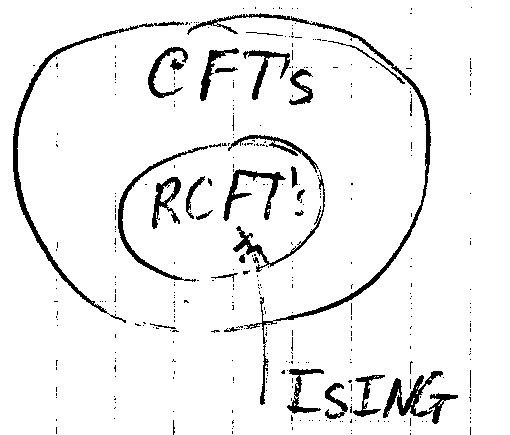
\includegraphics[width=\linewidth]{figures/gelfand-p001481-top-cft-sets-original.png}
\par\smallskip{\footnotesize Original manuscript diagram: GELFAND-P001481\par}
\end{minipage}\hfill
\begin{minipage}[c]{0.48\linewidth}\centering
\resizebox{\linewidth}{!}{% Partial visible-stroke recreation; uncertain connectivity remains open.
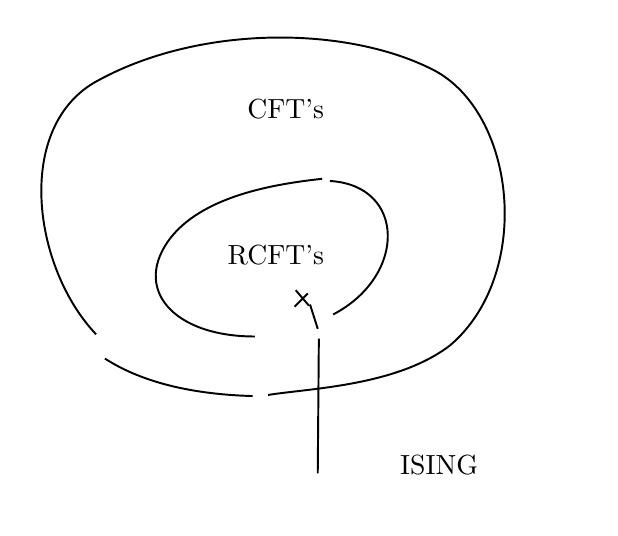
\begin{tikzpicture}[x=0.014cm,y=-0.014cm,line width=0.7pt]
\path[use as bounding box] (0,0) rectangle (510,435);
\draw (62,278)..controls(5,218)and(-12,93)..(60,50)
 ..controls(155,-4)and(293,-2)..(371,40)
 ..controls(444,82)and(457,225)..(383,288)
 ..controls(335,325)and(255,327)..(218,333);
\draw (204,334)..controls(135,332)and(95,316)..(70,300);
\draw (206,280)..controls(131,280)and(94,236)..(130,190)
 ..controls(162,150)and(232,141)..(267,137);
\draw (274,139)..controls(343,143)and(344,225)..(277,260);
\node at (234,74) {CFT's};\node at (225,206) {RCFT's};
\draw (263,404)--(264,282);\draw (263,273)--(256,251);
\draw (243,238)--(255,252);\draw (242,253)--(254,241);
\node at (373,397) {ISING};
\end{tikzpicture}
}
\par\smallskip{\footnotesize Partial recreation; unclear joins, crossings and arrowheads remain unresolved.\par}
\end{minipage}\par\medskip


R --- Rational

I [crossed out: \EnglishUnclear{GELFAND-P001481}{rational-cancelled-prefix}{illegible letters after I}]
\underline{RATIONAL.}\qquad (the name is historical)
$$
f(z_i,\tau_i,\bar z_i,\bar\tau_i)
=\sum_{j=1}^{N<\infty}\mathcal F_j(z_i,\tau_i)
\overline{\mathcal F}_j(\bar z_i,\bar\tau_i)
$$

\underline{Torus:}
$$\theta\to\theta+2\pi$$
$$\mathcal F_j(\tau)\ne\mathcal F_j(\tau+2\pi i)$$
$$\mathcal F_j(\tau)=\sum_\ell M_{j\ell}\mathcal F_\ell(\tau+2\pi i)$$
\EnglishUnclear{GELFAND-P001481}{torus-period-convention}{Both lines have $\tau+2\pi i$; at the bottom of this page is $T:\tau\to\tau+1$.}

$M=$ monodromy matrix.
[Crossed out: \EnglishUnclear{GELFAND-P001481}{monodromy-cancelled-word}{an illegible word}]

E.g. Ising
$$
Z(\tau,\bar\tau)=
\left|\sqrt{\frac{\theta_2}{\eta}}\right|^2+
\left|\sqrt{\frac{\theta_3}{\eta}}\right|^2+
\left|\sqrt{\frac{\theta_4}{\eta}}\right|^2
$$
$$\sqrt{\frac{\theta_2}{\eta}}=q^{1/8}\prod(1+q^n),\qquad q=e^{2\pi i\tau}$$
$$\sqrt{\frac{\theta_3}{\eta}}=\prod(1-q^{n-1/2})$$
$$\sqrt{\frac{\theta_4}{\eta}}=\prod(1+q^{n-1/2}).$$
\EnglishUnclear{GELFAND-P001481}{ising-product-conventions}{The exponent $1/8$, the minus sign in the $\theta_3$ line and the plus sign in the $\theta_4$ line are reproduced as in the source; the normalization is not specified.}

\underline{I.M.G.} Elliptic functions are trigonometry with parameter $q$.

$\mathcal F_j$ are not invariant, but $f$ is invariant

($\overline{\mathcal F}_j$
need not be complex conjugates of $\mathcal F_j$!)

A braid group arises.

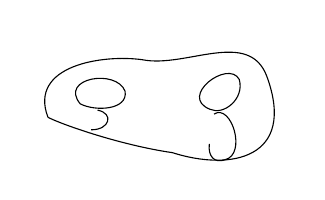
\begin{tikzpicture}[x=1cm,y=1cm]
\draw (0,.4) .. controls (-.25,1.06) and (.7,1.2) .. (1.2,1.13)
.. controls (1.75,1.02) and (2.55,1.53) .. (2.78,.92)
.. controls (3.16,-.12) and (2.33,-.29) .. (1.58,-.05)
.. controls (.89,.05) and (.12,.33) .. (0,.4);
\draw (.41,.57) .. controls (.14,.9) and (.87,1.02) .. (.98,.73)
.. controls (1.02,.49) and (.6,.47) .. (.41,.57);
\draw (2.06,.5) .. controls (1.65,.66) and (2.29,1.14) .. (2.43,.88)
.. controls (2.5,.63) and (2.23,.42) .. (2.06,.5);
\draw (.63,.49) .. controls (.84,.45) and (.79,.24) .. (.55,.24);
\draw (2.11,.44) .. controls (2.33,.58) and (2.53,-.07) .. (2.25,-.14)
.. controls (2.12,-.19) and (2.03,-.1) .. (2.05,.06);
\end{tikzpicture}

Generalize.

$g=1$
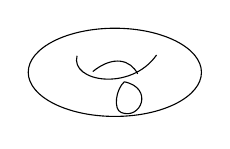
\begin{tikzpicture}[x=1cm,y=1cm]
\draw (0,0) ellipse (1.1cm and .56cm);
\draw (-.48,.21) .. controls (-.57,-.12) and (.2,-.25) .. (.53,.22);
\draw (-.28,.01) .. controls (-.02,.22) and (.2,.16) .. (.29,-.02);
\draw (.12,-.12) .. controls (.5,-.2) and (.33,-.61) .. (.08,-.51)
.. controls (-.02,-.47) and (.01,-.22) .. (.12,-.12);
\end{tikzpicture}
$$
S:\tau\to-1/\tau\qquad
T:\tau\to\tau+1
$$
$$S^2=1,\qquad (ST)^3=I$$

\EnglishSourceFrame{GELFAND-P001482}{unlabelled}
\underline{``DEHNTWIST''}

\underline{$g=2$}
\EnglishSourceFigure{GELFAND-P001482}{top-genus-two-twists}{A surface with two handles, with curves and labels $\alpha_1,\beta_1$ by the left handle, $\alpha_2$ along the middle part, and $\beta_2,\alpha_3$ by the right handle. Some curves overlap the edges of the holes; gaps and joins of strokes prevent confidently reconstructing every passage.}

\par\medskip\noindent
\begin{minipage}[c]{0.48\linewidth}\centering
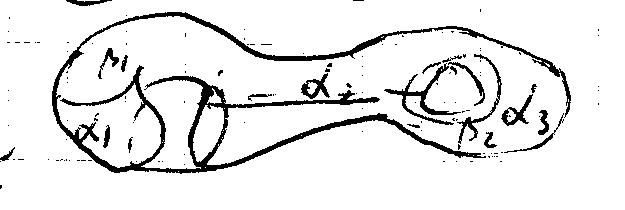
\includegraphics[width=\linewidth]{figures/gelfand-p001482-top-genus-two-twists-original.png}
\par\smallskip{\footnotesize Original manuscript diagram: GELFAND-P001482\par}
\end{minipage}\hfill
\begin{minipage}[c]{0.48\linewidth}\centering
\resizebox{\linewidth}{!}{% Partial visible-stroke recreation; uncertain connectivity remains open.
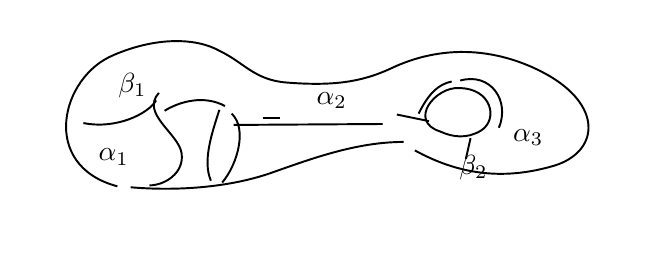
\begin{tikzpicture}[x=0.012cm,y=-0.012cm,line width=0.7pt]
\path[use as bounding box] (0,0) rectangle (625,210);
\draw (95,168)..controls(12,146)and(35,52)..(91,29)
 ..controls(135,10)and(178,10)..(204,25)
 ..controls(229,37)and(240,55)..(273,58)
 ..controls(322,62)and(353,58)..(385,43)
 ..controls(453,11)and(515,29)..(554,52)
 ..controls(610,86)and(603,132)..(558,146)
 ..controls(501,163)and(454,154)..(410,130);
\draw (398,121)..controls(348,121)and(300,139)..(260,153)
 ..controls(213,170)and(155,173)..(109,169);
\draw (145,88)..controls(161,78)and(187,71)..(209,83);
\draw (216,91)..controls(233,107)and(222,145)..(206,164);
\draw (139,69)..controls(119,91)and(160,112)..(163,133)
 ..controls(166,154)and(145,167)..(129,167);
\draw (203,87)..controls(195,112)and(185,141)..(194,162);
\draw (59,101)..controls(94,108)and(128,91)..(136,77);
\draw (218,103)--(376,102);\draw (249,96)--(267,96);
\draw (437,110)..controls(402,99)and(432,62)..(457,64)
 ..controls(491,64)and(499,97)..(480,109)
 ..controls(465,118)and(450,116)..(437,110);
\draw (414,91)..controls(425,69)and(435,60)..(449,57);
\draw (458,56)..controls(490,47)and(511,77)..(499,106);
\draw (391,92)--(425,99);\draw (469,117)--(464,139);
\node at (91,137) {$\alpha_1$};\node at (111,61) {$\beta_1$};
\node at (322,77) {$\alpha_2$};\node at (472,148) {$\beta_2$};
\node at (530,116) {$\alpha_3$};
\end{tikzpicture}
}
\par\smallskip{\footnotesize Partial recreation; unclear joins, crossings and arrowheads remain unresolved.\par}
\end{minipage}\par\medskip

$$z_i,\tau_i\to\tilde z_i,\tilde\tau_i$$

$$\alpha_1\beta_1\alpha_1=\beta_1\alpha_1\beta_1$$
$$\alpha_2\beta_2\alpha_2=\beta_2\alpha_2\beta_2$$
$$\alpha_2\beta_1\alpha_2=\beta_1\alpha_2\beta_1\qquad(\beta_1\to\beta_2)$$
$$\alpha_1\alpha_2=\alpha_2\alpha_1$$
$$\beta_1\beta_2=\beta_2\beta_1\qquad\text{etc.}$$
$$ (\alpha_1\beta_1\alpha_2)^4=\alpha_3^2 $$
$$ (\alpha_3\beta_2\alpha_2\beta_1\alpha_1^2\beta_1\alpha_2\beta_2\alpha_3)^2=1 $$
$$ \beta_1^{-1}\alpha_1\beta_1=\alpha_1\beta_1\alpha_1^{-1}. $$

[Two horizontal lines with a dot between them.]

CFT.
$$\mathcal A=\{(\sigma,\Delta)\ \text{fields}\}=\text{operator algebra}$$
$$\mathcal A\qquad\{T(z),T'(z),\ldots\}$$
$$
\mathcal H=\bigoplus_{i=1}^{N}
\underset{\mathcal A}{\mathcal H_i}\otimes
\underset{\bar{\mathcal A}}{\mathcal H_{\bar i}}
$$
$$\Delta:\mathcal A\to\mathcal A\otimes\mathcal A$$
$$ L_n=\oint_c\zeta^{n+1}T(\zeta) $$
$$ \to\oint\zeta^{n+1}T(\zeta)\otimes1+1\otimes\oint\zeta^{n+1}T(\zeta) $$
\EnglishUnclear{GELFAND-P001482}{ln-integration-symbol}{The variable resembles $\zeta$ or $\xi$; below the first contour integral is $c$ or $C$. No differential is written in these lines.}

$\rho_i:\mathcal A\to\operatorname{End}\mathcal H_i$,\qquad
\EnglishUnclear{GELFAND-P001482}{rho-trailing-fragment}{$\rho_i\,C$ or $\rho_i\,O$; a short fragment with no visible continuation}

[A separating line of small strokes.]

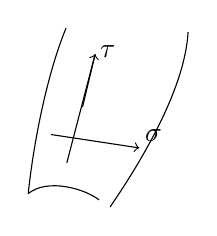
\begin{tikzpicture}[x=1cm,y=1cm]
\draw (0,0) .. controls (.08,.76) and (.27,1.6) .. (.48,2.1);
\draw (1.04,-.17) .. controls (1.49,.49) and (1.99,1.36) .. (2.03,2.05);
\draw (0,0) .. controls (.25,.2) and (.72,.06) .. (.9,-.08);
\draw (.49,.39)--(.85,1.77);
\draw[->] (.69,1.1)--(.85,1.77);
\draw[->] (.29,.75)--(1.41,.58);
\node at (1.01,1.8) {$\tau$};
\node at (1.59,.74) {$\sigma$};
\end{tikzpicture}
$$
S=\int g_{\mu\nu}(X)
[(\partial_\sigma X^\mu)(\partial_\sigma X^\nu)
-(\partial_\tau X^\mu)(\partial_\tau X^\nu)]
$$
Conformal Invariance $\to R_{\mu\nu}=0$.

\EnglishSourceFrame{GELFAND-P001483}{86}
\underline{I.M.G.} What should replace the notion of space upon quantization?

(the Planck length is $\sim 10^{-33}$ m)
\EnglishUnclear{GELFAND-P001483}{planck-unit}{The unit after $10^{-33}$ is m.}

\underline{First variant}: something discrete.

Riemann understood that this was important and thought through the notion of space.

A thin film near a 4-dimensional surface.

\underline{A reasonable exercise}: naive geometry of 4-dimensional polyhedra.

\begin{center}
\begin{tikzpicture}[x=1cm,y=1cm]
\draw (0,0) -- (0.75,-0.03);
\draw (1.07,0.01) -- (1.04,-0.12);
\draw (1.43,0.01) -- (2.47,-0.04);
\end{tikzpicture}
\end{center}

$$
S=\int_{R^4}g_{\mu\nu}(X)
\bigl[(\partial_\sigma X^\mu)(\partial_\sigma X^\nu)
-(\partial_\tau X^\mu)(\partial_\tau X^\nu)\bigr]+S_K
$$

[A brace beneath the integral term; below it and on the right:]
$$
\begin{array}{ccc}
c_{R^4}&+c_K=&26\\
\Vert&&\\
4&&
\end{array}
$$

[A short line leads from $S_K$ to the annotation:]
compact
\EnglishUnclear{GELFAND-P001483}{sk-annotation}{kond. na utolshch. pr-va / kond. na uplotn. pr-va / kond. na upolshch. pr-va / kond. na uploshch. pr-va [source abbreviations; four uncertain readings]}

can be replaced by $\forall$ other model with certain
invariance properties

$$
c\left(\begin{gathered}\text{conformal Field}\\\text{Theory}\end{gathered}\right)\text{ — }?
$$

[Below “Theory”, a short vertical line and the annotation “any”;
a brace leads up to “any” from the annotation on the left “also makes sense”.]

Therefore [crossed out:
\EnglishUnclear{GELFAND-P001483}{cft-cancellation}{has / have [source verb alternatives]}]
this is interesting.

\underline{19.9.88.}\qquad\underline{Gelfand's seminar.}

\underline{\underline{Morozov A.}}

\underline{Conformal field theory}
(based on Moore's talk).

String theory has been developing since 1984.

\underline{The initial picture}

\begin{center}
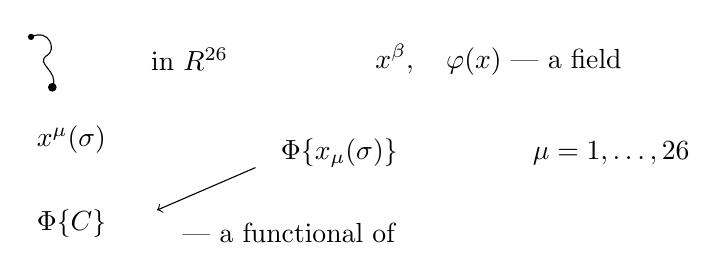
\begin{tikzpicture}[x=1cm,y=1cm]
\draw (0,2.14) .. controls (0.24,2.25) and (0.32,1.97) .. (0.21,1.91)
 .. controls (0.03,1.80) and (0.37,1.71) .. (0.27,1.50);
\fill (0,2.14) circle (0.04);
\fill (0.27,1.50) circle (0.055);
\node[anchor=west] at (1.40,1.85) {in $R^{26}$};
\node[anchor=west] at (4.25,1.85) {$x^\beta,\quad\varphi(x)$ --- a field};
\node[anchor=west] at (-0.05,0.83) {$x^\mu(\sigma)$};
\node[anchor=west] at (3.05,0.66) {$\Phi\{x_\mu(\sigma)\}$};
\node[anchor=west] at (6.25,0.66) {$\mu=1,\ldots,26$};
\node[anchor=west] at (-0.05,-0.23) {$\Phi\{C\}$};
\draw[->] (2.85,0.48) -- (1.60,-0.06);
\node[anchor=west] at (1.80,-0.35) {--- a functional of};
\end{tikzpicture}
\end{center}

\EnglishUnclear{GELFAND-P001483}{field-overwrite}{In the “field” line, the sign before $(x)$ is overwritten: $\varphi$ / $\Phi$.}
\EnglishUnclear{GELFAND-P001483}{contour-ending}{After “functional of”: a contour / contours; the word ending is overwritten.}

\begin{equation*}
(1)\quad
\langle\varphi(x_1)\ldots\varphi(x_n)\rangle
=\int D\varphi\,e^{\Sigma(\varphi)}\varphi(x_1)\ldots\varphi(x_n)
\end{equation*}

\EnglishUnclear{GELFAND-P001483}{eq1-first-symbol}{The first field sign in (1) is overwritten: $\varphi$ / $\Phi$.}

\EnglishSourceFigure{GELFAND-P001483}{particle-diagram}{Three lines labeled $x_1$, $x_2$, $x_3$ on the left. The upper line is wavy; the middle and lower lines rise to the right toward two places on the upper line. At the first place is a dark point; on the right is a dark point or arrowhead. The exact stroke connections at these places are unclear.}

\par\medskip\noindent
\begin{minipage}[c]{0.48\linewidth}\centering
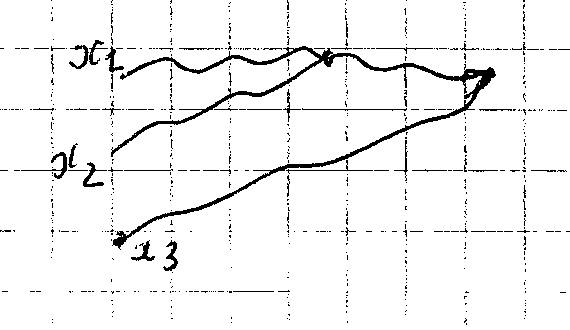
\includegraphics[width=\linewidth]{figures/gelfand-p001483-particle-diagram-original.png}
\par\smallskip{\footnotesize Original manuscript diagram: GELFAND-P001483\par}
\end{minipage}\hfill
\begin{minipage}[c]{0.48\linewidth}\centering
\resizebox{\linewidth}{!}{% Partial visible-stroke recreation; uncertain connectivity remains open.
\begin{tikzpicture}[x=0.014cm,y=-0.014cm,line width=0.7pt]
\path[use as bounding box] (0,0) rectangle (570,330);
\draw (126,78)..controls(161,55)and(166,52)..(187,66)
 ..controls(207,79)and(227,48)..(245,59)
 ..controls(265,72)and(287,46)..(302,48);
\draw (309,51)..controls(319,58)and(327,64)..(336,61)
 ..controls(367,56)and(370,78)..(395,69)
 ..controls(421,57)and(452,77)..(463,77);
\draw (117,151)..controls(157,124)and(182,126)..(198,120)
 ..controls(230,113)and(243,89)..(260,94)
 ..controls(286,104)and(302,81)..(321,65);
\draw (122,238)..controls(158,207)and(189,214)..(219,195)
 ..controls(253,176)and(278,165)..(305,166)
 ..controls(340,166)and(393,132)..(429,123)
 ..controls(457,117)and(471,98)..(480,82);
\draw[line width=1.3pt] (319,63)--(329,55);\draw[line width=1.3pt] (470,78)--(489,72);
\node at (90,49) {$x_1$};\node at (70,162) {$x_2$};\node at (157,260) {$x_3$};
\end{tikzpicture}
}
\par\smallskip{\footnotesize Partial recreation; unclear joins, crossings and arrowheads remain unresolved.\par}
\end{minipage}\par\medskip


(There were 3 particles at first; nothing remained at the end)

$\Sigma(\varphi)$ is called the quantum action

\EnglishSourceFrame{GELFAND-P001484}{unlabelled}
We want the same in string theory

\begin{equation*}
(2)\quad
\langle\Phi(C_1)\ldots\Phi(C_n)\rangle
\longrightarrow
\int D\Phi\,e^{\Sigma(\Phi)}\Phi(C_1)\ldots\Phi(C_n);
\end{equation*}

\EnglishUnclear{GELFAND-P001484}{eq2-relation}{The overwritten sign before the integral: $\longrightarrow$ / $\Rightarrow$ / $=$.}

but there is no reasonable progress in this direction!

But: the left-hand side of (2) can be described in other terms.

\begin{equation*}
(3)\quad
\Phi(C)=\sum\varphi_n(x)e^{in\sigma}\qquad(\text{closed string})
\end{equation*}

$\varphi_n$ are identified with the fields in (1)

Consider

\begin{equation*}
(4)\quad
\langle\varphi_{N_1}(x_1)\ldots\varphi_{N_n}(x_n)\rangle
\end{equation*}

and write another representation for it.

\begin{equation*}
(5)\quad
\langle\varphi(x_1)\varphi(x_2)\rangle
=\int Dx\,e^{-mL},\qquad
L=\int\sqrt{\dot{x}^2}\,dt
\end{equation*}

\EnglishUnclear{GELFAND-P001484}{eq5-exponent-overwrite}{In the exponent, the letter after the minus is overwritten; the visible reading is $-mL$, and the earlier strokes are illegible.}

[Below the left-hand side of (5), a vertical equals sign:]
$$
\begin{gathered}
\Vert\\
\int D\varphi\,e^{\Sigma_0(\varphi)}\varphi(x_1)\varphi(x_2)
\end{gathered}
$$

for the [inserted above: simplest] action $\Sigma_0$ describing a free particle.

\begin{equation*}
(6)\quad
\Sigma_0(\varphi)=\int(\partial\varphi)^2\partial^{26}x
+\int\varphi^3d^{26}x
\end{equation*}

\EnglishUnclear{GELFAND-P001484}{eq6-measure}{The first measure sign is $\partial$.}
\EnglishUnclear{GELFAND-P001484}{eq6-cubic-free}{The second term is $+\int\varphi^3d^{26}x$.}

Now

\begin{equation*}
(7)\quad
\langle\varphi_{N_1}(x_1)\ldots\varphi_{N_n}(x_n)\rangle
\sim\int Dx\,e^S\,V_{N_1}(x)\ldots V_{N_n}(x),
\end{equation*}

[Below the integral:]
over (nonsingular) world surfaces $x^\mu(\sigma,t)$
and over all topologies

$V_{N_j}$ are vertex operators
\EnglishUnclear{GELFAND-P001484}{vertex-index}{The small lower index beside $N$: $j$ / $d$.}

(8)
\EnglishSourceFigure{GELFAND-P001484}{branching-diagram}{A ribbon-like figure: an almost vertical edge on the left, curved upper and lower boundaries extending to a second nearly vertical line. Four curves diverge to the right, the two inner ones crossing. The exact joins of the boundaries to the second vertical line and the meaning of the crossing are unclear. On the right, a large curved arrow leads left from the area of the word “branchings” to the drawing.}

\par\medskip\noindent
\begin{minipage}[c]{0.48\linewidth}\centering
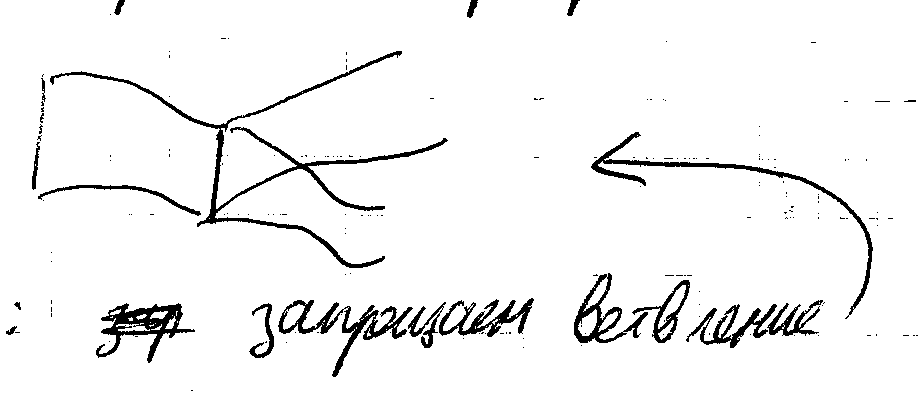
\includegraphics[width=\linewidth]{figures/gelfand-p001484-branching-diagram-original.png}
\par\smallskip{\footnotesize Original manuscript diagram: GELFAND-P001484\par}
\end{minipage}\hfill
\begin{minipage}[c]{0.48\linewidth}\centering
\resizebox{\linewidth}{!}{% Partial visible-stroke recreation; uncertain connectivity remains open.
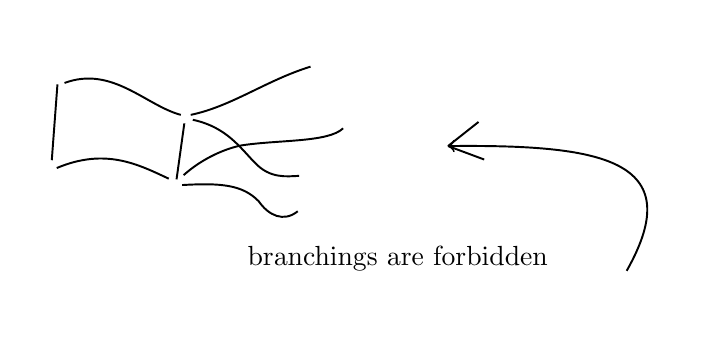
\begin{tikzpicture}[x=0.009cm,y=-0.009cm,line width=0.7pt]
\path[use as bounding box] (0,0) rectangle (920,400);
\draw (42,80)--(34,187);
\draw (52,78)..controls(119,53)and(167,110)..(216,123);
\draw (41,198)..controls(110,169)and(156,193)..(199,213);
\draw (221,135)--(210,214);
\draw (230,123)..controls(288,111)and(337,74)..(399,55);
\draw (233,130)..controls(281,140)and(301,171)..(321,191)
 ..controls(342,213)and(365,210)..(383,209);
\draw (220,208)..controls(248,183)and(281,170)..(302,166)
 ..controls(355,158)and(424,162)..(445,142);
\draw (218,222)..controls(271,219)and(303,221)..(326,245)
 ..controls(340,265)and(361,275)..(381,259);
\draw[->] (845,343)..controls(935,184)and(806,165)..(593,167);
\draw (593,167)--(636,133);\draw (593,167)--(644,186);
\node at (522,326) {branchings are forbidden};
\end{tikzpicture}
}
\par\smallskip{\footnotesize Partial recreation; unclear joins, crossings and arrowheads remain unresolved.\par}
\end{minipage}\par\medskip


String theory: [crossed out:
\EnglishUnclear{GELFAND-P001484}{branching-cancellation}{zap / zapr [source abbreviated beginnings]}]
branchings are forbidden

\begin{center}
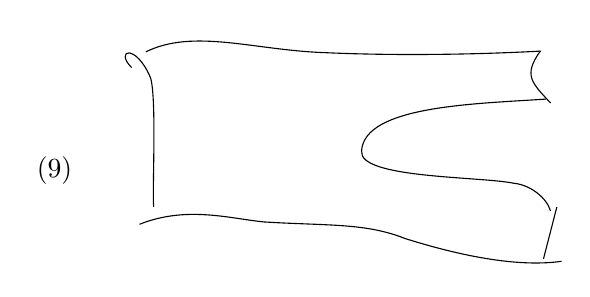
\begin{tikzpicture}[x=1cm,y=1cm]
\node[anchor=east] at (-0.55,1.12) {(9)};
\draw (0.26,2.63) .. controls (0.87,2.93) and (1.64,2.65) .. (2.53,2.62)
 .. controls (3.63,2.57) and (4.75,2.61) .. (5.28,2.64);
\draw (0.08,2.43) .. controls (-0.14,2.65) and (0.13,2.75) .. (0.32,2.30)
 .. controls (0.40,2.04) and (0.34,0.85) .. (0.36,0.66);
\draw (5.27,2.64) .. controls (5.05,2.33) and (5.16,2.24) .. (5.40,1.98);
\draw (5.34,2.03) .. controls (4.47,1.97) and (3.03,1.95) .. (3.00,1.37)
 .. controls (2.96,1.02) and (4.51,1.05) .. (4.94,0.96)
 .. controls (5.14,0.94) and (5.35,0.78) .. (5.40,0.61);
\draw (5.48,0.66) -- (5.31,0.00);
\draw (0.18,0.44) .. controls (0.78,0.68) and (1.34,0.51) .. (1.76,0.47)
 .. controls (2.56,0.42) and (3.05,0.46) .. (3.55,0.26)
 .. controls (4.09,0.09) and (4.91,-0.12) .. (5.54,-0.03);
\end{tikzpicture}
\end{center}

(but such transformations remain!)

and a theory of free particles results.

